\chapter{Ensemble methods} \label{cahpEnsemble}

%citazione introduttiva
\epigraph{\textit{A choir sings better than a single voice.}}{}


In the chapter \ref{cahpNonLinear} we introduced machine learning methods born from different research approaches. Each of them has peculiarity and limits, and there is not the best method that outperforms the others. Ensemble learning aims at combining the power of these different learners to obtain a more effective result. The idea behind ensemble learning is to combine different prediction models and consider their output together to make predictions on the target variable. Ensemble methods are mainly based on bagging and boosting (see Figure \ref{fig_ensemble}). Bagging combines the effect of multiple independent learners while boosting create a pipeline of learners in sequence.\footnote{The package logproj provides methods to deal with ensemble methods \href{https://github.com/aletuf93/logproj/blob/master/logproj/M_learningMethod/ensemble_methods.py}{here}.}

% INSERT fig_ensemble
\begin{figure}[hbt!]
\centering
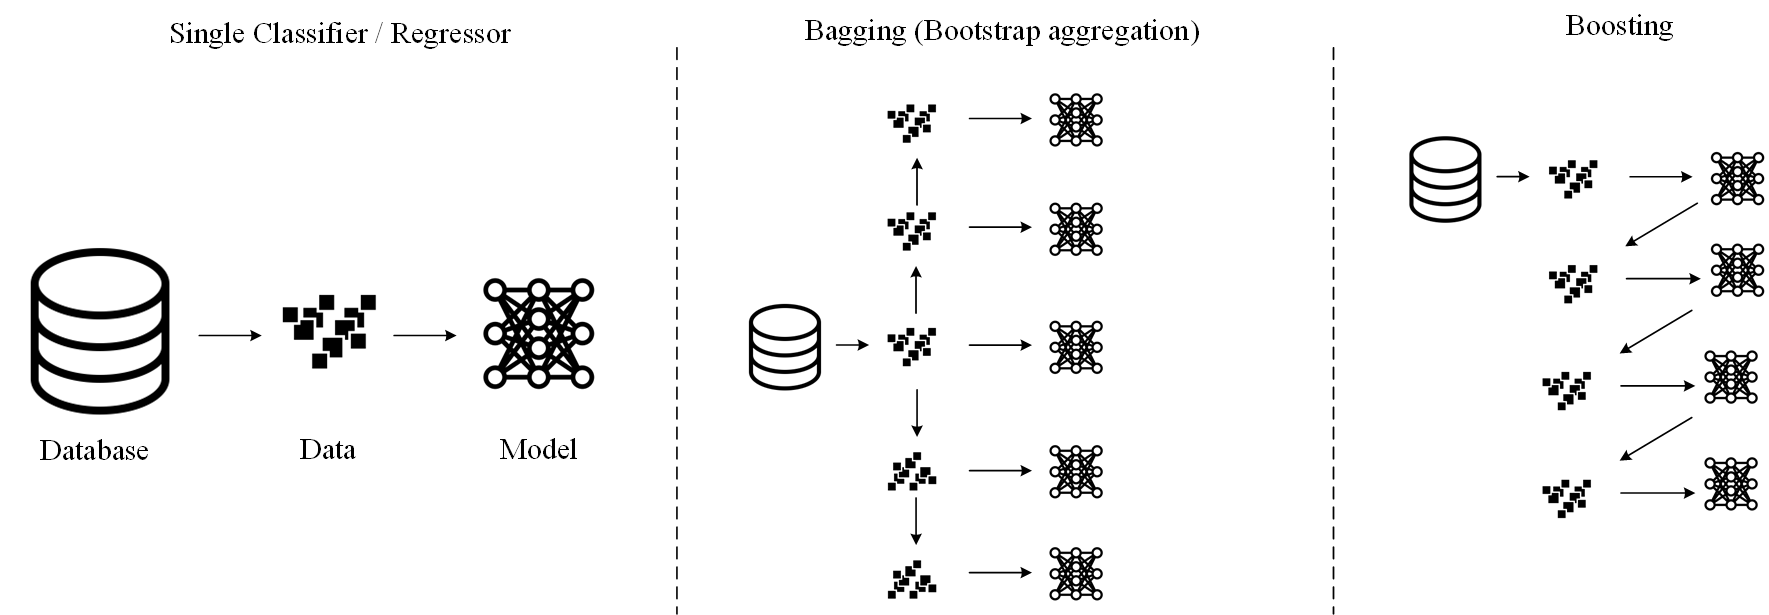
\includegraphics[width=1\textwidth]{SectionLetsMath/ensembleMethods_fig/fig_ensemble.png}
\captionsetup{type=figure}
\caption{Representation of the rationale of the ensemble methods.}
\label{fig_ensemble}
\end{figure}

\section{Bagging}
The word \textit{bagging} means \textit{bootstrap aggregation}. This method uses the bootstrap sampling technique (see section \ref{secBootstrapping}) to get $B$ different samples of the original dataset and train $B$ different models on them. The type of model to train can be chosen arbitrarily. The final prediction will be the average of the prediction $f^b$ of the $B$ models.

\begin{equation}
f\left(x\right)=\frac{1}{B}\sum_{b=1}^{B}{f^b(x)}
\label{eq_bagging}
\end{equation}

\section{Random Forests}
A Random Forest is a bagging method whose model is a decision tree or a regression tree. The underlying idea is to average many unbiased trees to reduce the variance in the predictions. Random forests work as follows.

\begin{algorithm}[H]
\DontPrintSemicolon
\SetAlgoLined
Import the input dataset with $N$ observations, and $p$ features\;
Set the number of iterations $B$\;
\For{$b=1:B$}{
    Get a bootstrap sample $Z^\ast$ of size $N$\;
    Set a number $m$ of features to extract\;
    Grow a tree tree $T_b$ on $Z^\ast$ doing the following\;
    \While{ a minimum node size $n_{min}$ is not reached.}
        {
            	Select $m$ variables out of $p$ at random\;
            	Choose the best variable split on $m$\;
            	Split the node into two daughter nodes\;
        }
}
Output the ensemble of trees ${T_1,\ldots,T_B}$\;

\caption{Random forests algorithm}
\label{algo_randomForest}
\end{algorithm}

Predictions are obtained differently depending on regression or classification. The predictions for a regression tree are obtained by averaging all the output predictions:

\begin{equation}
f\left(x\right)=\frac{1}{B}\sum_{b=1}^{B}{T_b\left(x\right)}
\label{eq_randomRegression}
\end{equation}

For a classification tree the function of majority vote is considered:

\begin{equation}
 f\left(x\right)=majority\ vote\ \left\{C_1\left(x\right),\ldots C_B(x)\right\} 
\label{eq_randomClassification}
\end{equation}

where $C_b(x)$ is the class predicted by the $b$ tree of the random forest.\par

The hyperparameters of a random forest are the number $m$ of features to extract and the minimum number of nodes $n_min$. Valid tuning parameter for regression random forests are $m=\sqrt p$, and $n_{min}=1$; while for classification random forests are used $m=p/3$, and $n_{min}=5$.\par

The performance of a random forest can be assessed through a traditional error metric (e.g. the MSE) calculated on out-of-bag (OOB) samples. OOB samples are the samples of the original dataset which does not appear in the bootstrapped dataset. This measure of error is similar to the cross-validation.

\section{AdaBoost}
\textit{AdaBoost} means adaptive boosting, and it has been one of the firsts boosting methods. The main idea behind these methods is to combine the outputs of many \textit{weak} classifiers to get a robust prediction. A weak classifier is any classification function with an error rate slightly better than random classification (i.e., flipping a coin). These \textit{weak} classifiers are called \textit{stumps}, and can be modelled as decision trees with a single split. Each of the classifiers votes to produce a different weighted contribution on the final prediction. AdaBoost born as a classification method on two classes $y\in{-1;1}$. The final prediction is obtained as:

\begin{equation}
G\left(x\right)=sign\left(\sum_{m=1}^{M}{\alpha_mG_m\left(x\right)}\right)
\label{eq_adaboost}
\end{equation}

Where $G_m(x)$ is the contribution of each weak predictor and $\alpha_1,\ldots,\alpha_m$ are the relative importance of each predictor. The AdaBoost algorithm works as follows:

\begin{algorithm}[H]
\DontPrintSemicolon
\SetAlgoLined

	Set a weight $w_i=\frac{1}{N}$ for each observation $i=1,\ldots,N$ \;
	\For{$m=1:M$}{
	    	Normalise weights $w_i$  $i=1,\ldots,N$ \;
	    	Fit a stump classifier $G_m(x)$ to the training data \;
	    	Compute the error $err_m=\frac{\sum_{i=1}^{N}{w_iI(y_i\neq G_m(x_i))}}{\sum_{i=1}^{N}w_i}$ \;
	    	Compute $\alpha_m=\log{\left(\frac{1-err_m}{err_m}\right)}$ \;
	        Set $w_i=w_ie^{\alpha_mI\left(y_i\neq G_m\left(x_i\right)\right)}\ i=1,\ldots,N$ \;
	  
	
	}
	Predict the output $G\left(x\right)=sign\left(\sum_{m=1}^{M}{\alpha_mG_m\left(x\right)}\right)$ \; 


\caption{AdaBoost algorithm}
\label{algo_adaboost}
\end{algorithm}

At each iteration, the algorithm increases the value of $\alpha_m$ if the classifier $G_m$ gives a robust prediction. In addition, a higher weight $w_i$ is associated with misclassified observation to give them higher importance in the forthcoming iterations. From this perspective, AdaBoost connects a series of stump classifiers as a chain such that the following classifiers produce good predictions where the previous failed.

\section{Gradient boosting}
Gradient boosting is a boosting model similar to AdaBoost with a main difference; it uses decision trees instead of stumps. Gradient boosting minimises a loss function $L\left(f\right)=\sum_{i=1}^{N}L\left(y_i,f\left(x_i\right)\right)$,  where $f(x)$ is a sum of trees. Algorithm \ref{algo_gradientBoosting} illustrates how gradient boosting works.


\begin{algorithm}[H]
\DontPrintSemicolon
\SetAlgoLined

    Initialise $f_0\left(x\right)=\arg{\min_\gamma{\sum_{i=1}^{N}L\left(y_i,\gamma\right)}}$ \;
	\For{$m=1:M$}{
    	\For{ observation $i=1:N$}{
    	    		$r_{im}=-\left[\left(\frac{\partial L\left(y_i,f\left(x_i\right)\right)}{\partial f\left(x_i\right)}\right)\right]_{f=f_{m-1}}$ \;
    	
    	}
	    Fit a tree with target $r_{im}$ and terminal regions $R_{jm}$, $j=1,\ldots,J_m$	\;
	    \For{ $j=1:J_m$}{
    	    		$\gamma_{jm}=\arg{\min_\gamma{\sum_{x_i\in R_{jm}}{L(y_i,f_{m-1}\left(x_i\right)+\gamma)}}}$ \;
    	}
    	Set $f_m\left(x\right)=f_{m-1}\left(x\right)+\rho\sum_{j=1}^{J_m}{\gamma_{jm}\left(x\in R_{jm}\right)}$
	  
	
	}
    Predict the output $\hat{f}\left(x\right)=f_M(x)$ \; 

\caption{AdaBoost algorithm}
\label{algo_gradientBoosting}
\end{algorithm}

In particular, working with a regression problem, the initial value is set to the average of the target variable $f_0\left(x\right)=\bar{y}$. The loss function $L=\frac{1}{2}\left(y_i-f\left(x_i\right)\right)^2$ is set to the sum of squared residual multiplied by a coefficient $\frac{1}{2} $which will be simplified after calculating the gradient of $L$. \par

The algorithm builds $M$ different trees to get the final prediction. Each tree defines $J_m$ terminal regions (i.e. leaves) to target the value of $r_{im}$. The value of $r_{im}$ is calculated at each step, based on the value of the loss function $L$ generated at the previous tree $f_{m-1}$. The values of $f_m$, i.e. the prediction on $y$ at the step $m$ of the algorithm, is generated summing the prediction from the previous step $f_{m-1}$ plus a value $\gamma_{jm}$. $\gamma_{jm}$ is the output value at the terminal region $R_{jm}$ chosen to minimise the sum of squared residuals generated by the multiple observations falling into the same leave $R_{jm}$. $\rho\in[0,1]$ is a learning rate used to reduce the variance produced by the model on the test set. The experience suggests setting the hyperparameters choosing $\rho=0.1$ and building trees with 8 to 32 leaves. \par

Gradient boosting can be used for classification problem as well, by setting the initial value equal to the log of the odds of the target variable. The algorithm updates the values of the $\gamma_{jm}$ with respect to the residuals of the predicted values calculated on a logistic function. 


\section{Mixture of Experts}
The \textit{mixture of experts} models combine the predictions of multiple trees in a soft way (see Section \ref{secClustering}). As the word \textit{mixture} suggests, this is not a hard model, but it works by calculating the probability that a point belongs to a split branch or another. The terminal nodes of this tree are called \textit{experts}, while the non-terminal nodes are \textit{gating networks}. Gating networks have an output in the form:

\begin{equation}
g_j\left(x,\gamma_j\right)=\frac{e^{\gamma_j^Tx}}{\sum_{k=1}^{K}e^{\gamma_k^Tx}}\ j=1,\ldots,K
\label{eq_mixtureOfExperts1}
\end{equation}

Where $g_j\left(x,\gamma_j\right)$ represents the probability of assigning a vector $x$ of the input dataset to the branch $j$. $\gamma_j$ is a vector of unknown parameters representing the soft $k$-way split (while dealing with regression tree $k$ is always equal to 2). At each terminal node (expert), the response variable is in the form:

\begin{equation}
Y \sim \Pr(y|x,\theta_{jl})
\label{eq_mixtureOfExperts2}
\end{equation}

Where $Y$ is a linear regression model $\theta_{jl}=(\beta_{jl},\sigma_{jl}^2)$. $Y=\beta_{jl}^Tx+\epsilon\ \sim N(0,\sigma_{jl}^2)$. In the case of classification, $Y$ is the logistic regression. 
